\documentclass{article}

\usepackage{natbib}
\usepackage[utf8]{inputenc}
\usepackage[english]{babel}
\usepackage{natbib}
\usepackage{hyperref}
\usepackage{adjustbox}
\bibliographystyle{apalike}

\title{Ecological performance of detecting data fabrication with summary statistics}
\author{Chris HJ Hartgerink, Jelte M Wicherts, Marcel ALM van Assen}

\usepackage{Sweave}
\begin{document}
\input{manuscript-concordance}
\maketitle


\section*{Study 1}


We tested the performance of statistical methods to detect data fabrication based on summary results with genuine and fabricated summary results of four anchoring studies \citep{tversky1974,jacowitz1995}. The anchoring effect is a well-known psychological heuristic that uses the information in the question as the starting point for the answer, which is then adjusted to yield a final estimate of a quantity. For example 'Is the percentage of African countries in the United Nations more or less than [10\% or 65\%]?'. These questions yield mean responses of 25\% and 45\%, respectively \citep{tversky1974}, despite essentially posing the same factual question. A considerable amount of genuine datasets on this heuristic are freely available and we collected fabricated datasets within this study.

\subsection*{Methods}

The four anchoring studies for which results were collected were (i) distance from San Francisco to New York, (ii) population of Chicago, (iii) height of the Mount Everest, and (iv) the number of babies born per day in the United States. Each of the four studies provided summary results for a 2 (low/high anchoring) $\times$ 2 (male/female) factorial design. Throughout this study, the unit of analysis is a set of summary statistics (i.e., means, standard deviations, and test results) for the four anchoring studies from one respondent. For current purposes, a respondent is defined as researcher/lab where the four anchoring studies' summary statistics originate from. All materials, data, and analyses scripts are freely available on the OSF (\url{osf.io/b24pq}) and were preregistered (\url{osf.io/ejf5x}; deviations are explicated in this report).

\subsubsection*{Data collection}

We downloaded thirty-six genuine datasets from the publicly available Many Labs (ML) project \citep[\url{osf.io/pqf9r};][]{klein2014}. The ML project replicated several effects across thirty-six locations, including the anchoring effect in the four studies mentioned previously. Considering the size of the ML project, the transparency of research results, and minimal individual gain for fraud, we assumed these data to be genuine. For each of the thirty-six locations, sample sizes, means, and standard deviations (four each) were computed for each of the four conditions in the four anchoring studies across the thirty-six locations (i.e., $3\times4\times4\times36$). We computed these summary statistics from the raw ML data, which were cleaned using the original analysis scripts from the ML project.

Using quotum sampling, we collected thirty-six fabricated datasets of summary results for all four anchoring studies. Quotum sampling was applied to sample as many responses as possible for the available 36 rewards (i.e., not all respondents might request the gift card and count towards the quotum; one participant did not request a reward). The sampling frame consisted of 2,038 psychology researchers who published a peer-reviewed paper in 2015, as indexed in the Web of Science (WoS) with the filter set to the U.S. We sampled psychology researchers to improve familiarity with the anchoring effect \citep{jacowitz1995,tversky1974}, for which summary results were fabricated. We filtered for U.S. researchers to ensure familiarity with the imperial measurement system, which is the scale of some of the anchoring studies (note: we found out several non-U.S. researchers were included because this filter also retained papers with co-authors from the U.S.). WoS was searched on October 13, 2015. In total, 2,038 unique corresponding e-mails were extracted from 2,014 papers (due to multiple corresponding authors).

A random sample of 1,000 researchers were approached via e-mail to participate in this study on April 25, 2016 (invitation: \url{osf.io/s4w8r}). The study took place via Qualtrics with anonimization procedures in place (e.g., no IP-addresses saved). We informed the participating researchers that the study would require them to fabricate data and explicitly mentioned that we would investigate these data with statistical methods to detect data fabrication. We also clarified to the  respondents that they could stop at any time without providing a reason. If they wanted, respondents received a \$30 Amazon gift card as compensation for their participation if they were willing to enter their email address. They could win an additional \$50 Amazon gift card if they were one of three top fabricators. The provided email addresses were unlinked from individual responses upon sending the bonus gift cards. The full text of the Qualtrics survey is available at \url{osf.io/w984b}.

Each respondent was instructed to fabricate 32 summary statistics (4 studies $\times$ 2 conditions $\times$ 2 sexes $\times$ 2 statistics [mean and sd]) that fulfilled three hypotheses. We instructed respondents to fabricate results for the hypotheses (i) main effect of condition, (ii) no effect of sex, and (iii) no interaction effect between condition and sex. Respondents did not need to fabricate sample sizes, which were set to 25 per cell a priori. The fabricated summary statistics and their accompanying test results for these three hypotheses serve as the data to examine the properties of tools to detect data fabrication.

We provided respondents with a template spreadsheet to fill out the fabricated data, in order to standardize the fabrication process without restraining the participant in how they chose to fabricate data. Figure \ref{fig1} depicts an example of this spreadsheet (original:  \url{osf.io/w6v4u}). We requested respondents to fill in the yellow cells with fabricated data, which includes means and the standard deviations for four conditions. Using these values, statistical tests are computed and shown in the "Current result" column instantaneously. If these results confirmed the hypotheses, a checkmark appeared as depicted in Figure \ref{fig1}. We required respondents to copy-paste the yellow cells into Qualtrics, to provide a standardized response format that could be automatically processed in the analyses.

\begin{figure}
\begin{center}
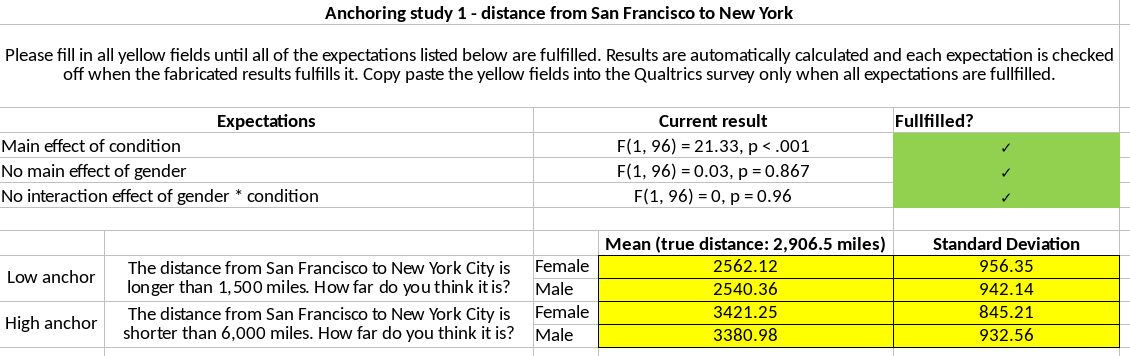
\includegraphics[width=\textwidth,height=\textheight,keepaspectratio]{../figures/spreadsheet.png}
\caption{Example of a filled in template spreadsheet used in the fabrication process. Respondents fabricated data in the yellow cells, which were used to compute the results of the hypothesis tests. If the fabricated data confirm the hypotheses, a checkmark appeared in a green cell.}
\label{fig1}
\end{center}
\end{figure}

Upon completing the fabrication of the data, respondents were debriefed. Respondents answered several questions about their statistical knowledge and approach to data fabrication and finally we reminded them that data fabrication is widely condemned by professional organizations, institutions, and funding agencies alike. We rewarded participation with a \$30 Amazon gift card and the fabricated results that were most difficult to detect received a bonus \$50 Amazon gift card.

\subsubsection*{Data analysis}

To detect data fabrication in a set of summary results, we first tested the standardized standard deviations (SDs) for data fabrication \citep{simonsohn2013} across the four anchoring studies. This method tests whether the observed SDs contain a reasonable amount of variation, as expected based on random sampling processes. For example, if four independent samples all yield the variance $2.22$, this could be considered excessively consistent when the probability that this amount of consistency (or more) is less than 1 out of 1000 in truly random samples. To compute this probability, we first standardized the SDs for each of the four studies with
\begin{equation}
z_j=\sqrt{\frac{s^2_j}{MS_w}}=\sqrt{\frac{s^2_j}{\left(\frac{\sum\limits^k_{j=1}(N_j-1)s^2_j}{\sum\limits^k_{j=1}(N_j-1)}\right)}}
\label{s2_j}
\end{equation}
where $z_j$ denotes the standardized SD in group $j$ ($MS_w$ is the simple arithmetic mean when sample sizes are equal for all cells, which is the case for the fabricated datasets). We tested different measures to detect data fabrication that utilize these standardized SDs (i.e., $z_j$). We included the variance of the standardized SDs \citep[i.e.,  $SD_{z}$;][]{simonsohn2013} and tried out the max-min distance of the standardized SDs (denoted $max-min_{z}$) as an alternative measure. We compared the observed value for each measure with the expected distribution when the summary results are used to generate random samples. To this end, we simulated the expected distribution of standardized SDs and computed the expected distribution of each measure. This expected distribution was used to determine the $p$-value of the observed $SD_z$ and $max-min_z$. We simulated the standardized variance for each of the $j$ groups as
\begin{equation}
z^2_j\sim\left(\frac{\chi^2_{N_j-1}}{N_j-1}\right)/MS_w
\label{simvar}
\end{equation}
These simulated values are used to compute the expected distribution of the $SD_z$ and $max-min_z$  measures.

Testing the standardized SDs for potential data fabrication can be done either for each study separately or all studies combined; the test can also be done under different assumptions of population variances across conditions. The assumptions of population variance can either by that all SDs originate from the same distribution \citep[as in][]{simonsohn2013}, the SDs within a factor are from the same distribution, or each group comes from its own distribution. We preregistered the method that assumes the SDs are drawn from the same distribution for the various conditions (i.e., homogeneous SDs) and are tested across all studies. However, upon conducting the analyses, we decided homogenous SDs are not unequivocal and included computations where the SDs for the low anchor and high anchor are from different distributions (i.e., heterogeneous SDs). Additionally, the signal for data fabrication across the four anchoring studies might result in different studies cancelling each other out, so we also included analyses where each study was analyzed separately.

Second, we applied the reversed Fisher method to detect data fabrication to the nonsignificant $p$-values twice: once for the results of gender effects hypothesis in each study and once for the results of the interaction effect hypothesis for each study. The Fisher method \citep{fisher1925} tests for evidence of an effect in a set of $p$-values by testing for a right-skew $p$-value distribution, but we adjusted it here to test for results that are overly consistent with the null hypothesis and result in a left-skew distribution (see Figure \ref{leftskew}). The original Fisher method is computed as
\begin{equation}
\chi^2_{2k}=-2\sum\limits^k_{i=1}\ln(p_i)
\label{fishertest}
\end{equation}
and tests for right-skew in a set of $p$-values, but we adjust it to the following
\begin{equation}
\chi^2_{2k}=-2\sum\limits^k_{i=1}\ln(1-\frac{p_i-t}{1-t})
\label{fisheradjusted}
\end{equation}
where it now tests for left-skew (i.e., more larger $p$-values than smaller $p$-values) across the $k$ number of $p$-values that falls above the threshold $t$. We set this threshold to .05 in order to include only nonsignificant test results.


% add plot of left and right skew
\begin{figure}[!ht]
\begin{center}
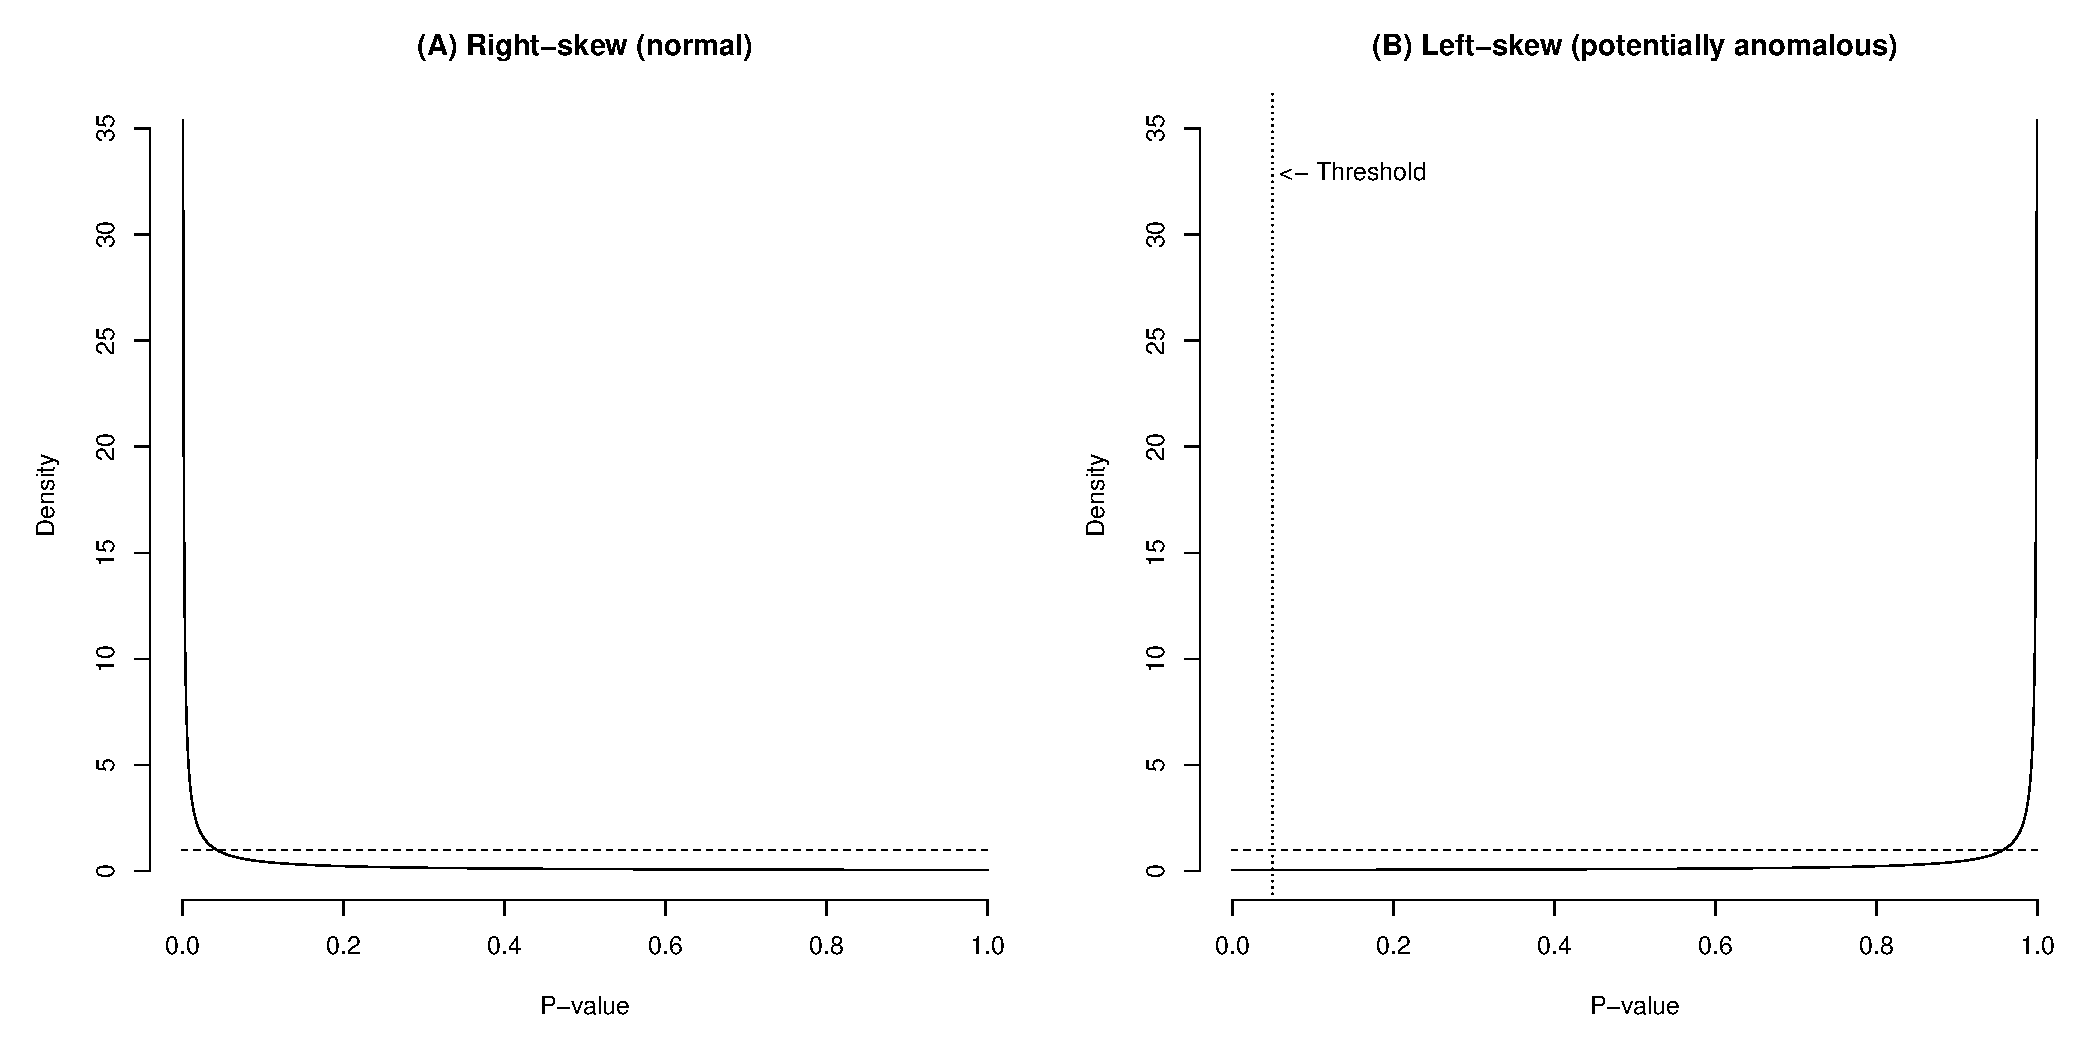
\includegraphics[width=\textwidth,height=\textheight,keepaspectratio]{../figures/fisherfig.pdf}
\caption{Conceptual representation of what the Fisher test inspects (Equation \ref{fishertest}; panel A) and what the adjusted Fisher test inspects (Equation \ref{fisheradjusted}; panel B). Both panels test whether there is sufficient evidence that the solid line deviates from the dashed line, except that the type of deviation that the test is sensitive to is the exact opposite.}
\label{leftskew}
\end{center}
\end{figure}

Finally, we combined the three methods to detect data fabrication into an overall detection method (i.e., combination method). This included the $SD_z$ measure across all studies and the Fisher test (Equation \ref{fisheradjusted}) of the gender hypothesis test and the interaction test.  We expected this combination test of the three individual tests for data fabrication to be more powerful than the individual tests, given that these tests inspect different manifestations of data fabrications. Based on the results of the combined test results, the three least detectable data fabricators were selected. The three respondents with the highest $p$-values on this combined method to detect data fabrication contained the least evidential value for deviating from genuine data and received an additional \$50 Amazon gift card.

For each of these four tests to detect data fabrication ($SD_z$, Fisher test for the gender and interaction hypotheses, combination method) we carried out sensitivity and specificity analyses using ROC-curves. With these ROC-curves, more informed decisions about optimal alpha levels can be made. In order to determine the optimal alpha level, we varied the alpha level from .000001 through .1. The optimal alpha level was determined by finding that alpha level for which the combination of true positive rate (TPR) and the true negative rate (TNR) were highest. For example, if $\alpha=.04$ results in $TPR=.30$ and $TNR=.7$, but $\alpha=.05$ results in $TPR=.5$ and $TNR=.5$, then .05 was chosen as an optimal decision criterion based on the sample.

\subsection*{Results}


The collected data included 36 genuine data from Many Labs 1 \citep[\url{osf.io/pqf9r};][]{klein2014} and 39 fabricated datasets(\url{osf.io/e6zys}). 3 participants did not participate for a bonus. Figure \ref{densities} shows a group-level comparison of the genuine- and fabricated $p$-values and effect sizes ($r$). Such group-level comparisons provide a general idea of the differences between the genuine- and fabricated data \citep[see also][]{Akhtar-Danesh2003}. 

% add plot of left and right skew
\begin{figure}[!ht]
\begin{center}
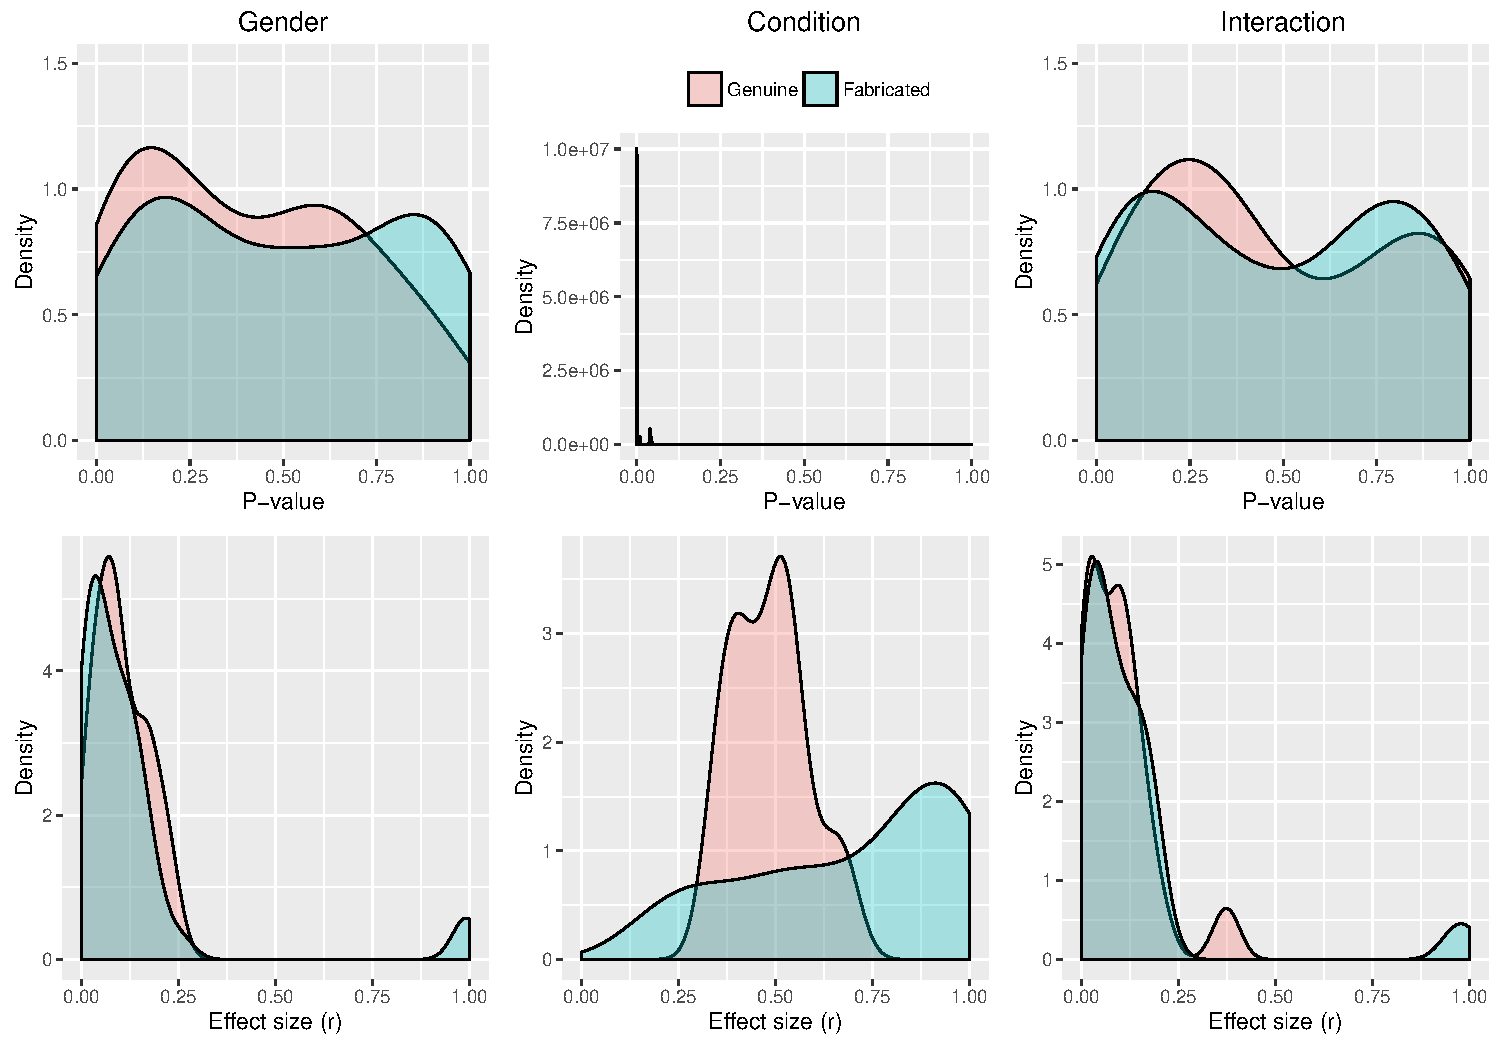
\includegraphics[width=\textwidth,height=\textheight,keepaspectratio]{../figures/ddfab_density.pdf}
\caption{Overlay of density distributions for both genuine and fabricated data, per effect and type of result. We instructed respondents to fabricate nonsignificant data for the gender and interaction effects, and a significant effect for the condition effect.}
\label{densities}
\end{center}
\end{figure}

The distributions in Figure \ref{densities} indicate little difference between genuine- and fabricated data when nonsignificant effects are inspected (i.e., gender and interaction hypotheses) whereas there seem to be large differences when subjects were required to fabricate significant data (i.e., condition hypothesis). From our own experience, and anecdotal evidence elsewhere \citep{BAILEY1991741}, large effects have raised initial suspicions previously. These data confirm that extremely large effect sizes (e.g., $r>.95$) might prove to be an easy-to-implement flag for potentially anomalous data (it is wise to seek for alternative explanations after flagging, nonetheless). Considering this, we also investigated how well effect sizes perform in detecting data fabrication (not preregistered).


\subsubsection*{Performance of using SDs to detect data fabrication}

% latex table generated in R 3.3.1 by xtable 1.8-2 package
% Thu Sep  1 17:46:56 2016
\begin{table}[ht]
\centering
\begin{tabular}{lrr}
  \hline
Method & $SD_z$ & $maxmin_z$ \\ 
  \hline
Homogeneous combined & 0.423 & 0.303 \\ 
  Homogeneous study 1 & 0.368 & 0.374 \\ 
  Homogeneous study 2 & 0.421 & 0.446 \\ 
  Homogeneous study 3 & 0.510 & 0.521 \\ 
  Homogeneous study 4 & 0.540 & 0.542 \\ 
  Heterogeneous combined & 0.770 & 0.756 \\ 
  Study 1 low condition & 0.643 & 0.643 \\ 
  Study 1 high condition & 0.438 & 0.438 \\ 
  Study 2 low condition & 0.751 & 0.751 \\ 
  Study 2 high condition & 0.612 & 0.612 \\ 
  Study 3 low condition & 0.668 & 0.668 \\ 
  Study 3 high condition & 0.651 & 0.651 \\ 
  Study 4 low condition & 0.796 & 0.796 \\ 
  Study 4 high condition & 0.555 & 0.555 \\ 
   \hline
\end{tabular}
\caption{Area Under the Curve (AUC) for the two statistical methods used to detect data fabrication based on variances. Homogeneous: assumes one population variance underlying all groups. Heterogeneous: assumes separate population variance per anchoring condition.} 
\label{auc_variances}
\end{table}


\begin{figure}[!ht]
\begin{center}
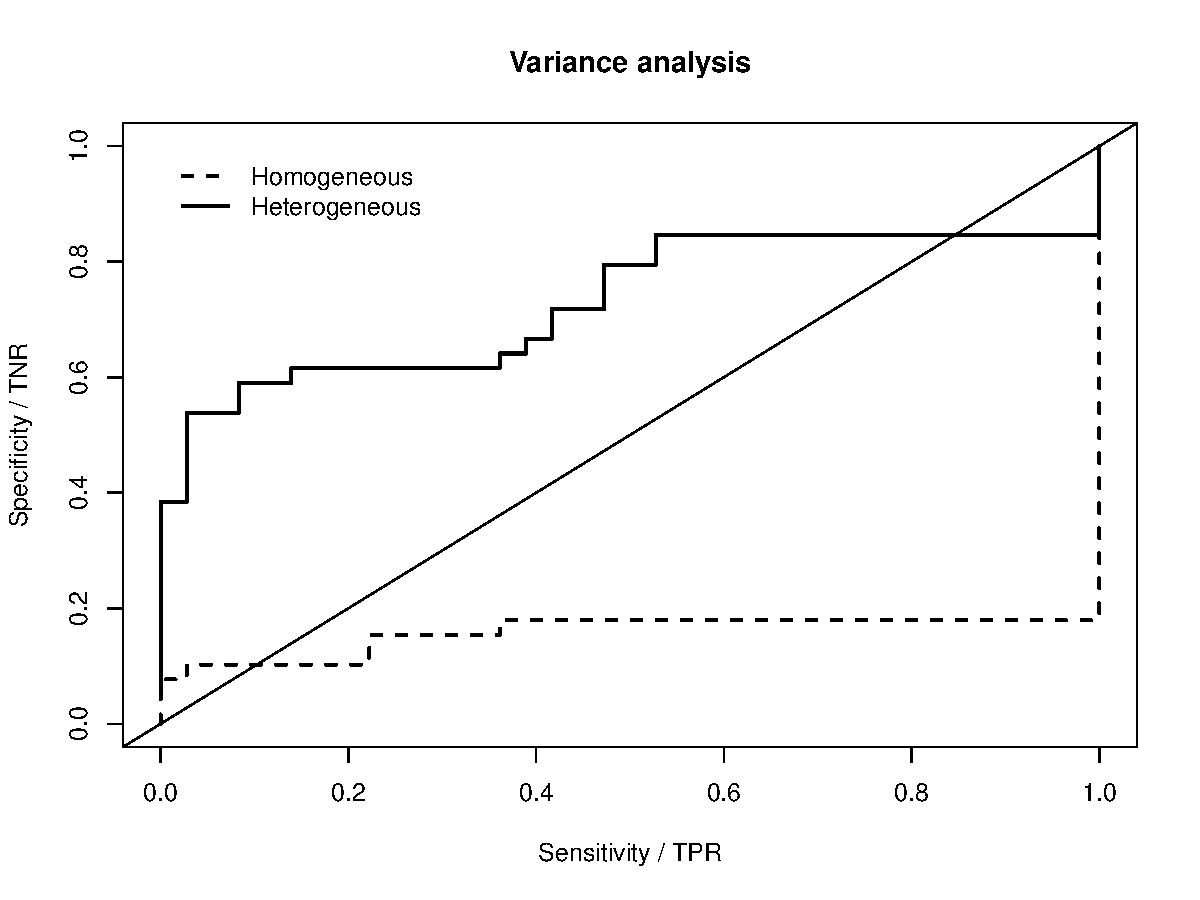
\includegraphics[width=\textwidth,height=\textheight,keepaspectratio]{../figures/varianceplot.pdf}
\caption{PLACEHOLDER}
\label{varianceplot}
\end{center}
\end{figure}

\subsubsection*{Performance of using $p$-values to detect data fabrication}

We asked researchers to fabricate data for nonsignificant effect sizes after inspecting whether the genuine data resembled a uniform distribution. Consequently, our hypothesis was that researchers who fabricate data would be unlikely to fabricate a uniform $p$-value distribution, given many researchers misinterpret the $p$-value (e.g., as the probability of an effect %REF
). However, as Table \ref{auc_fisher} indicates, the AUC for these methods are hardly better than chance. In other words, for effects that are specifically fabricated to be nonsignificant, researchers might not fabricate such large $p$-values to be suspicious.

% latex table generated in R 3.3.1 by xtable 1.8-2 package
% Thu Sep  1 17:46:56 2016
\begin{table}[ht]
\centering
\begin{tabular}{lr}
  \hline
Method & AUC \\ 
  \hline
Fisher test gender hypothesis & 0.521 \\ 
  Fisher test interaction hypothesis & 0.535 \\ 
   \hline
\end{tabular}
\caption{Area Under the Curve (AUC) for PLACEHOLDER} 
\label{auc_fisher}
\end{table}
\subsubsection*{Performance of combining SDs and $p$-value methods to detect data fabrication}


% latex table generated in R 3.3.1 by xtable 1.8-2 package
% Thu Sep  1 17:46:56 2016
\begin{table}[ht]
\centering
\begin{tabular}{lr}
  \hline
Method & AUC \\ 
  \hline
Combined Fisher test (3 results, $SD_z$ homogeneous) & 0.602 \\ 
  Combined Fisher test (3 results, $SD_z$ heterogeneous) & 0.736 \\ 
  Combined Fisher test (6 results, $SD_z$ homogeneous) & 0.643 \\ 
  Combined Fisher test (6 results, $SD_z$ heterogeneous) & 0.643 \\ 
   \hline
\end{tabular}
\caption{Area Under the Curve (AUC) for PLACEHOLDER} 
\label{auc_combined}
\end{table}

\subsubsection*{Performance of large effect sizes to detect data fabrication}


%The 23 largest significant effects were fabricated, with 13 (0.333\%) larger than $r=.9$. Based on descriptive data throughout psychology \citep{Hartgerink2016-lg}, effect sizes $\geq.9$ belong to the 96th percentile of effects throughout the psychology literature and effect sizes $\geq.95$ 98th percentile.


\subsection*{Discussion}

% variance analysis and effect size best ways to inspect
% but severely correlated: smaller variances = larger effects
% easiest way is too look for massive effects in the effects

% Simonsohn method not invalid under homogeneous, just somethign to take into account
% easily adjusted

% Discuss how the PPV is likely to be overestimated because prevalence is 50% in this study
% How we don't know the prevalence, in fact.


\bibliography{../bibliography/library}
\newpage
%------------------------------------
%handy to include this at the end
%------------------------------------
\section*{SessionInfo}
%-------------------------------------

\begin{Schunk}
\begin{Sinput}
> sessionInfo()
\end{Sinput}
\begin{Soutput}
R version 3.3.1 (2016-06-21)
Platform: x86_64-redhat-linux-gnu (64-bit)
Running under: Fedora 23 (Workstation Edition)

locale:
 [1] LC_CTYPE=en_US.UTF-8       LC_NUMERIC=C              
 [3] LC_TIME=en_US.UTF-8        LC_COLLATE=en_US.UTF-8    
 [5] LC_MONETARY=en_US.UTF-8    LC_MESSAGES=en_US.UTF-8   
 [7] LC_PAPER=en_US.UTF-8       LC_NAME=C                 
 [9] LC_ADDRESS=C               LC_TELEPHONE=C            
[11] LC_MEASUREMENT=en_US.UTF-8 LC_IDENTIFICATION=C       

attached base packages:
[1] stats     graphics  grDevices utils     datasets  methods   base     

other attached packages:
 [1] stringr_1.0.0   plyr_1.8.4      car_2.0-19      httr_1.2.0     
 [5] xtable_1.8-2    gridExtra_2.2.1 ggplot2_2.1.0   latex2exp_0.4.0
 [9] foreign_0.8-66  pROC_1.8       

loaded via a namespace (and not attached):
 [1] Rcpp_0.12.6      MASS_7.3-45      R6_2.1.2         grid_3.3.1      
 [5] gtable_0.2.0     magrittr_1.5     scales_0.4.0     stringi_1.1.1   
 [9] tools_3.3.1      munsell_0.4.3    colorspace_1.2-6 nnet_7.3-12     
\end{Soutput}
\begin{Sinput}
> 
\end{Sinput}
\end{Schunk}

\end{document}
